% IEEE conference template for the final project report.
% Overleaf: New Project > Blank Project, replace main.tex with this file, Recompile.
% IEEEtran is built into Overleaf. No other files are needed until real figures are added.

\documentclass[conference]{IEEEtran}

\usepackage[T1]{fontenc} % also gives the Times font when compiling locally with Tectonic
\usepackage{cite}
\usepackage{amsmath,amssymb,amsfonts}
\usepackage{graphicx}
\usepackage{textcomp}
\usepackage{array}
\usepackage{flafter}
\usepackage{tikz}
\usetikzlibrary{positioning,arrows.meta}

% Table settings: L{width} and C{width} are left-aligned and centred columns of a fixed width.
\newcolumntype{L}[1]{>{\raggedright\arraybackslash}p{#1}}
\newcolumntype{C}[1]{>{\centering\arraybackslash}p{#1}}
\renewcommand{\arraystretch}{1.2}

% Figure placeholder: \figplaceholder{height}{what the figure will show}.
% To add a real figure, replace the \figplaceholder line in that figure with:
%   \includegraphics[width=\linewidth]{file_name.png}
\newcommand{\figplaceholder}[2]{%
  \fbox{\parbox[c][#1][c]{\dimexpr\linewidth-2\fboxsep-2\fboxrule\relax}{\centering\footnotesize #2}}}

\begin{document}

% Working title. It may change.
\title{Benchmarking LLMs against Navigation Tools}

\author{\IEEEauthorblockN{Ishan Kaustubh Mehta}
\IEEEauthorblockA{\textit{Department of Computer Science}\\
\textit{BITS Pilani, K K Birla Goa Campus}\\
Goa, India\\
email address}
% To add a co-author, remove the % signs on the next four lines.
% \and
% \IEEEauthorblockN{Vinayak Naik}
% \IEEEauthorblockA{\textit{Department of Computer Science}\\
% \textit{BITS Pilani, K K Birla Goa Campus}\\ Goa, India\\ email address}
}

\maketitle

\begin{abstract}
We build a memory-efficient ETL (extract, transform, load) pipeline that turns Bangalore's official lists of major roads into traffic readings from Google's Routes API. [Rest of the abstract: the question, the comparison, the main results and what they mean. Write this last.]
\end{abstract}

\begin{IEEEkeywords}
Four to six search terms for the topic, method and city.
\end{IEEEkeywords}

% ======================================================================
\section{Introduction}

Navigation tools such as Google Maps answer questions like ``how long will it take to drive from A to B at 6~pm?'' by combining a detailed road map with live and historical traffic data. Large language models (LLMs) are now asked the same kind of question in everyday chat, but they have no map and no traffic feed: whatever they answer comes from the text they saw during training. How much of a city's roads and traffic such a model has absorbed is not obvious, and a confident but wrong travel time is easy to believe.

Bangalore is a demanding place to test this. Its traffic changes strongly over the day, and the same road often goes by more than one name. This paper asks: \emph{how close can LLMs, using only their own knowledge, get to Google Maps on routes, distances and travel times in Bangalore?} We split this into five smaller questions:
\begin{enumerate}
\item Do the models know where well-known places are and which roads exist?
\item How close are their distances and travel times to Google's?
\item Do they know when traffic is heavy?
\item On which trips are they worst?
\item How much does the wording of the prompt change their answers?
\end{enumerate}

Answering these needs reliable reference data and a fair way to ask a navigation tool and an LLM the same question (Fig.~\ref{fig:overview}). We first collected data from Google Maps in two ways. An ETL (extract, transform, load) pipeline turned the city's official lists of major roads into traffic readings taken every two hours for a week, which show when and where traffic is heavy. Google's predicted travel times for the benchmark trips then serve as the reference answers. The benchmark itself asks Google Maps, Gemini and ChatGPT about 72 trips between named landmarks, each at four times on every day of a week.

Our contributions are:
\begin{itemize}
\item a benchmark that gives Google Maps and the LLMs the same 2,016 trip queries, with whole-route and road-by-road answers;
\item a comparison of Gemini and ChatGPT with Google Maps on places, roads, distances and travel times;
\item a check of how prompt wording and answer format shift an LLM's travel-time estimates;
\item a memory-efficient ETL pipeline from official road lists to traffic readings, used to choose the benchmark routes and a baseline.
\end{itemize}

Section~II reviews related work. Section~\ref{sec:gmaps} describes the Google Maps data: the city-wide traffic data and the reference answers for the benchmark. Section~\ref{sec:design} describes the benchmark design and Section~\ref{sec:results} the results. Section~\ref{sec:discussion} discusses the results and their limits, and Section~\ref{sec:conclusion} concludes.

\begin{figure}[!htb]
\centering
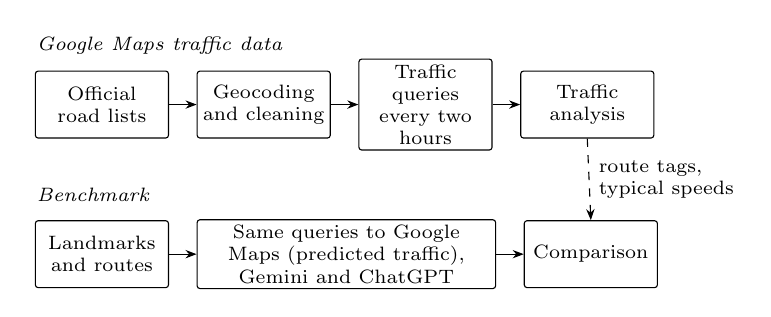
\begin{tikzpicture}[
  box/.style={draw, rounded corners=1pt, align=center, font=\scriptsize, minimum height=0.85cm, text width=1.55cm, inner sep=2pt},
  arr/.style={-{Stealth[length=4pt]}, thin},
  lab/.style={font=\scriptsize\itshape}]
\node[lab, anchor=west] (t1) at (-0.95,0.75) {Google Maps traffic data};
\node[box] (a1) at (0,0) {Official road lists};
\node[box, right=0.35cm of a1] (a2) {Geocoding and cleaning};
\node[box, right=0.35cm of a2] (a3) {Traffic queries every two hours};
\node[box, right=0.35cm of a3] (a4) {Traffic analysis};
\draw[arr] (a1) -- (a2); \draw[arr] (a2) -- (a3); \draw[arr] (a3) -- (a4);
\node[lab, anchor=west] (t2) at (-0.95,-1.15) {Benchmark};
\node[box] (b1) at (0,-1.9) {Landmarks and routes};
\node[box, right=0.35cm of b1, text width=3.65cm] (b2) {Same queries to Google Maps (predicted traffic), Gemini and ChatGPT};
\node[box, right=0.35cm of b2] (b4) {Comparison};
\draw[arr] (b1) -- (b2);
\draw[arr] (b2) -- (b4);
\draw[arr, dashed] (a4.south) -- node[right, font=\scriptsize, align=left]{route tags,\\typical speeds} (b4.north);
\end{tikzpicture}
\caption{Overview. Google Maps traffic data on the main roads supplies the route tags and typical speeds used in the benchmark, where Google Maps also gives the reference answers.}
\label{fig:overview}
\end{figure}

% ======================================================================
\section{Related Work}

Several studies ask what LLMs know about geography. Gurnee and Tegmark~\cite{gurnee2024} found that the internal activations of Llama-2 models encode where places are, at world, country and city scale. Bhandari et al.~\cite{bhandari2023} probed smaller models for the coordinates of cities and concluded that useful geographic knowledge needs larger models, and Manvi et al.~\cite{manvi2024} showed that adding OpenStreetMap context to a prompt helps LLMs predict quantities such as population density. These works test where places are, not how to travel between them.

Closer to our question, Roberts et al.~\cite{roberts2023} tested GPT-4 on geographic tasks that include route planning and compared some of its routes with those of Google Maps. Chen et al.~\cite{chen2024} asked GPT-4, Gemini and Mistral to plan real driving and walking routes from a university campus and found many errors in every scenario. MapEval~\cite{dihan2025} scores models on 700 map-based multiple-choice questions across 180 cities; no model passed 67\,\% accuracy, and distances and routes were among the weakest areas. Guo et al.~\cite{guo2026} trained an LLM on 13 million transit route records from four Chinese cities to plan routes without a map. To our knowledge, none of these compares an LLM's distances and travel times with a navigation tool's predictions across the hours and days of a week in one city, which is what our benchmark does.

Two further studies shape our design. Akbar et al.~\cite{akbar2023} measured travel speed and congestion in 180 Indian cities from trips simulated with a web mapping service, which supports using such a service as a source of city traffic data. Sclar et al.~\cite{sclar2024} showed that small changes in prompt format can change LLM results considerably and recommended reporting results across formats; our comparison of prompt wordings and answer formats follows this advice.

% ======================================================================
\section{Google Maps Data}\label{sec:gmaps}

Google Maps plays two roles in this work. It is the reference that the LLMs are scored against, and before the benchmark it was our source for understanding how traffic moves in Bangalore. We therefore collected two kinds of data from it. The first is a city-wide set of traffic readings on the main roads, taken every two hours for a week. It shows when and where traffic is heavy, and we use it to choose benchmark routes that cover changeable roads and to set the speeds of a simple baseline. The second is Google's answer to every benchmark query, the ground truth for the results in Section~\ref{sec:results}.

\subsection{City-Wide Traffic Data}\label{sec:traffic_data}
The Bruhat Bengaluru Mahanagara Palike (BBMP), the city's municipal body, publishes lists of 80 arterial and 285 sub-arterial roads as PDF files. We typed them into one table and wrote each road as a chain of places: its origin, the places it passes and its destination. Names that cannot be placed on a map, such as ``Ring Road'' or ``BBMP Limit'', were removed with a short blocklist, as were names containing ``Road'' without a landmark word such as ``Cross'' or ``Circle''. The rest were converted to coordinates with the Google Geocoding API. Of the 365 roads, 87 kept fewer than two located places and were dropped. Two overlap rules, applied to coordinates rounded to about 11~m, removed five more: of two routes with the same ends we kept the one with more places in between, and a route lying wholly inside a longer one was dropped. This left 273 routes, 74 arterial and 199 sub-arterial (Fig.~\ref{fig:route_geometries}).

\begin{figure}[!htb]
\centering
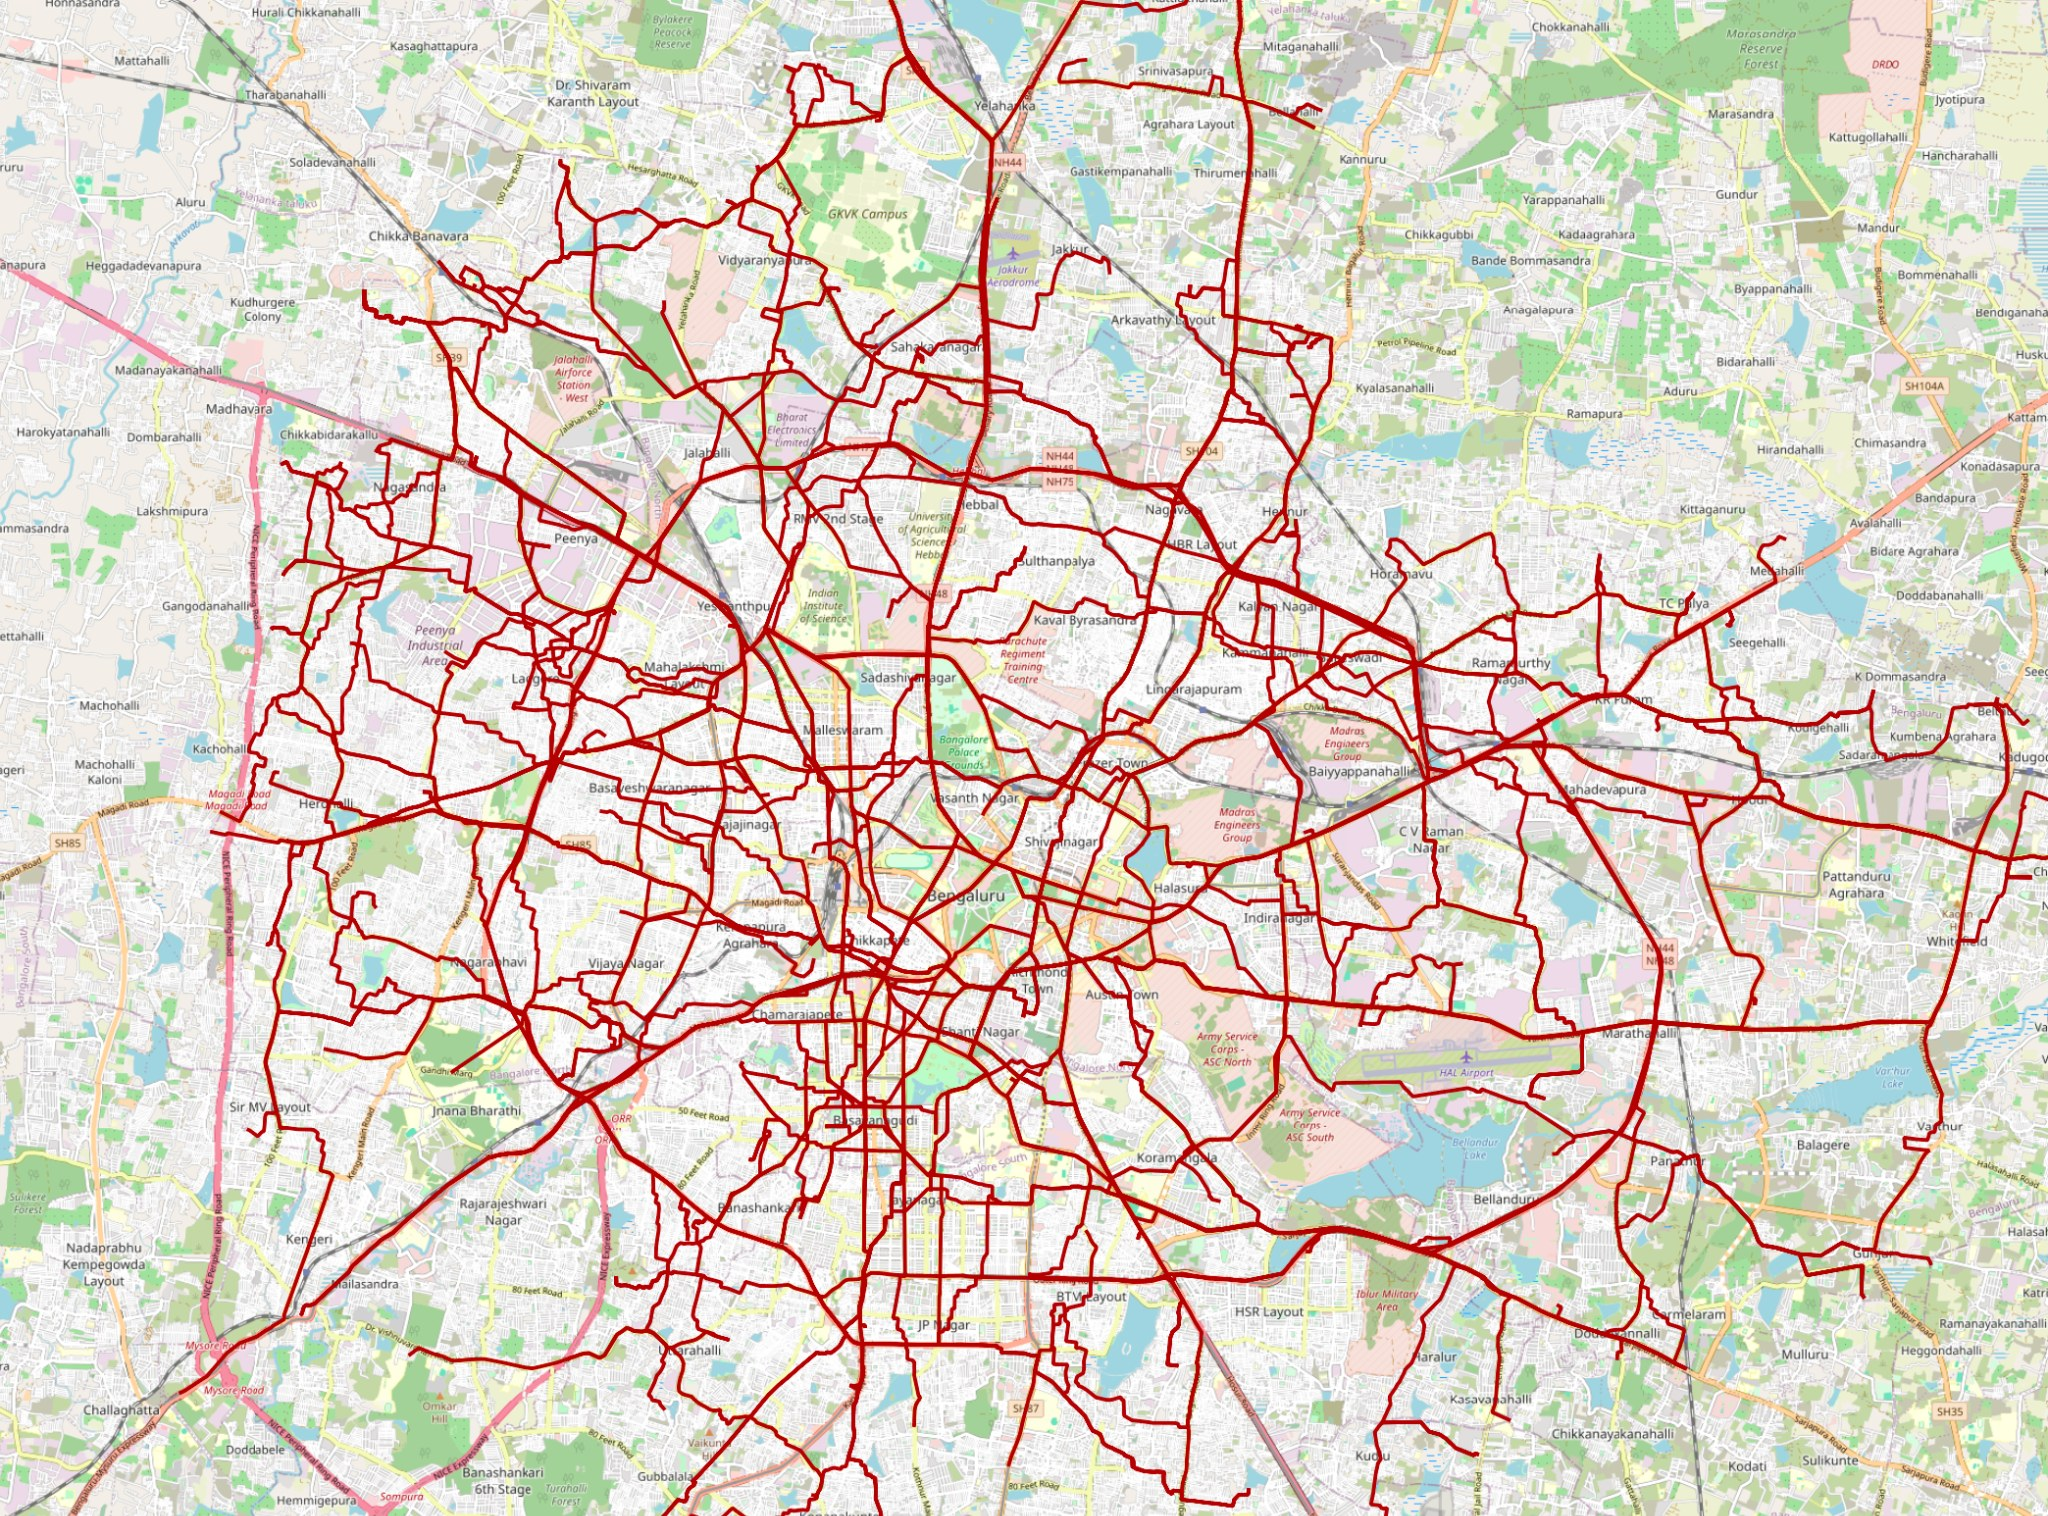
\includegraphics[height=3.4cm]{figures/fig_routes_arterial.jpg}\hfill
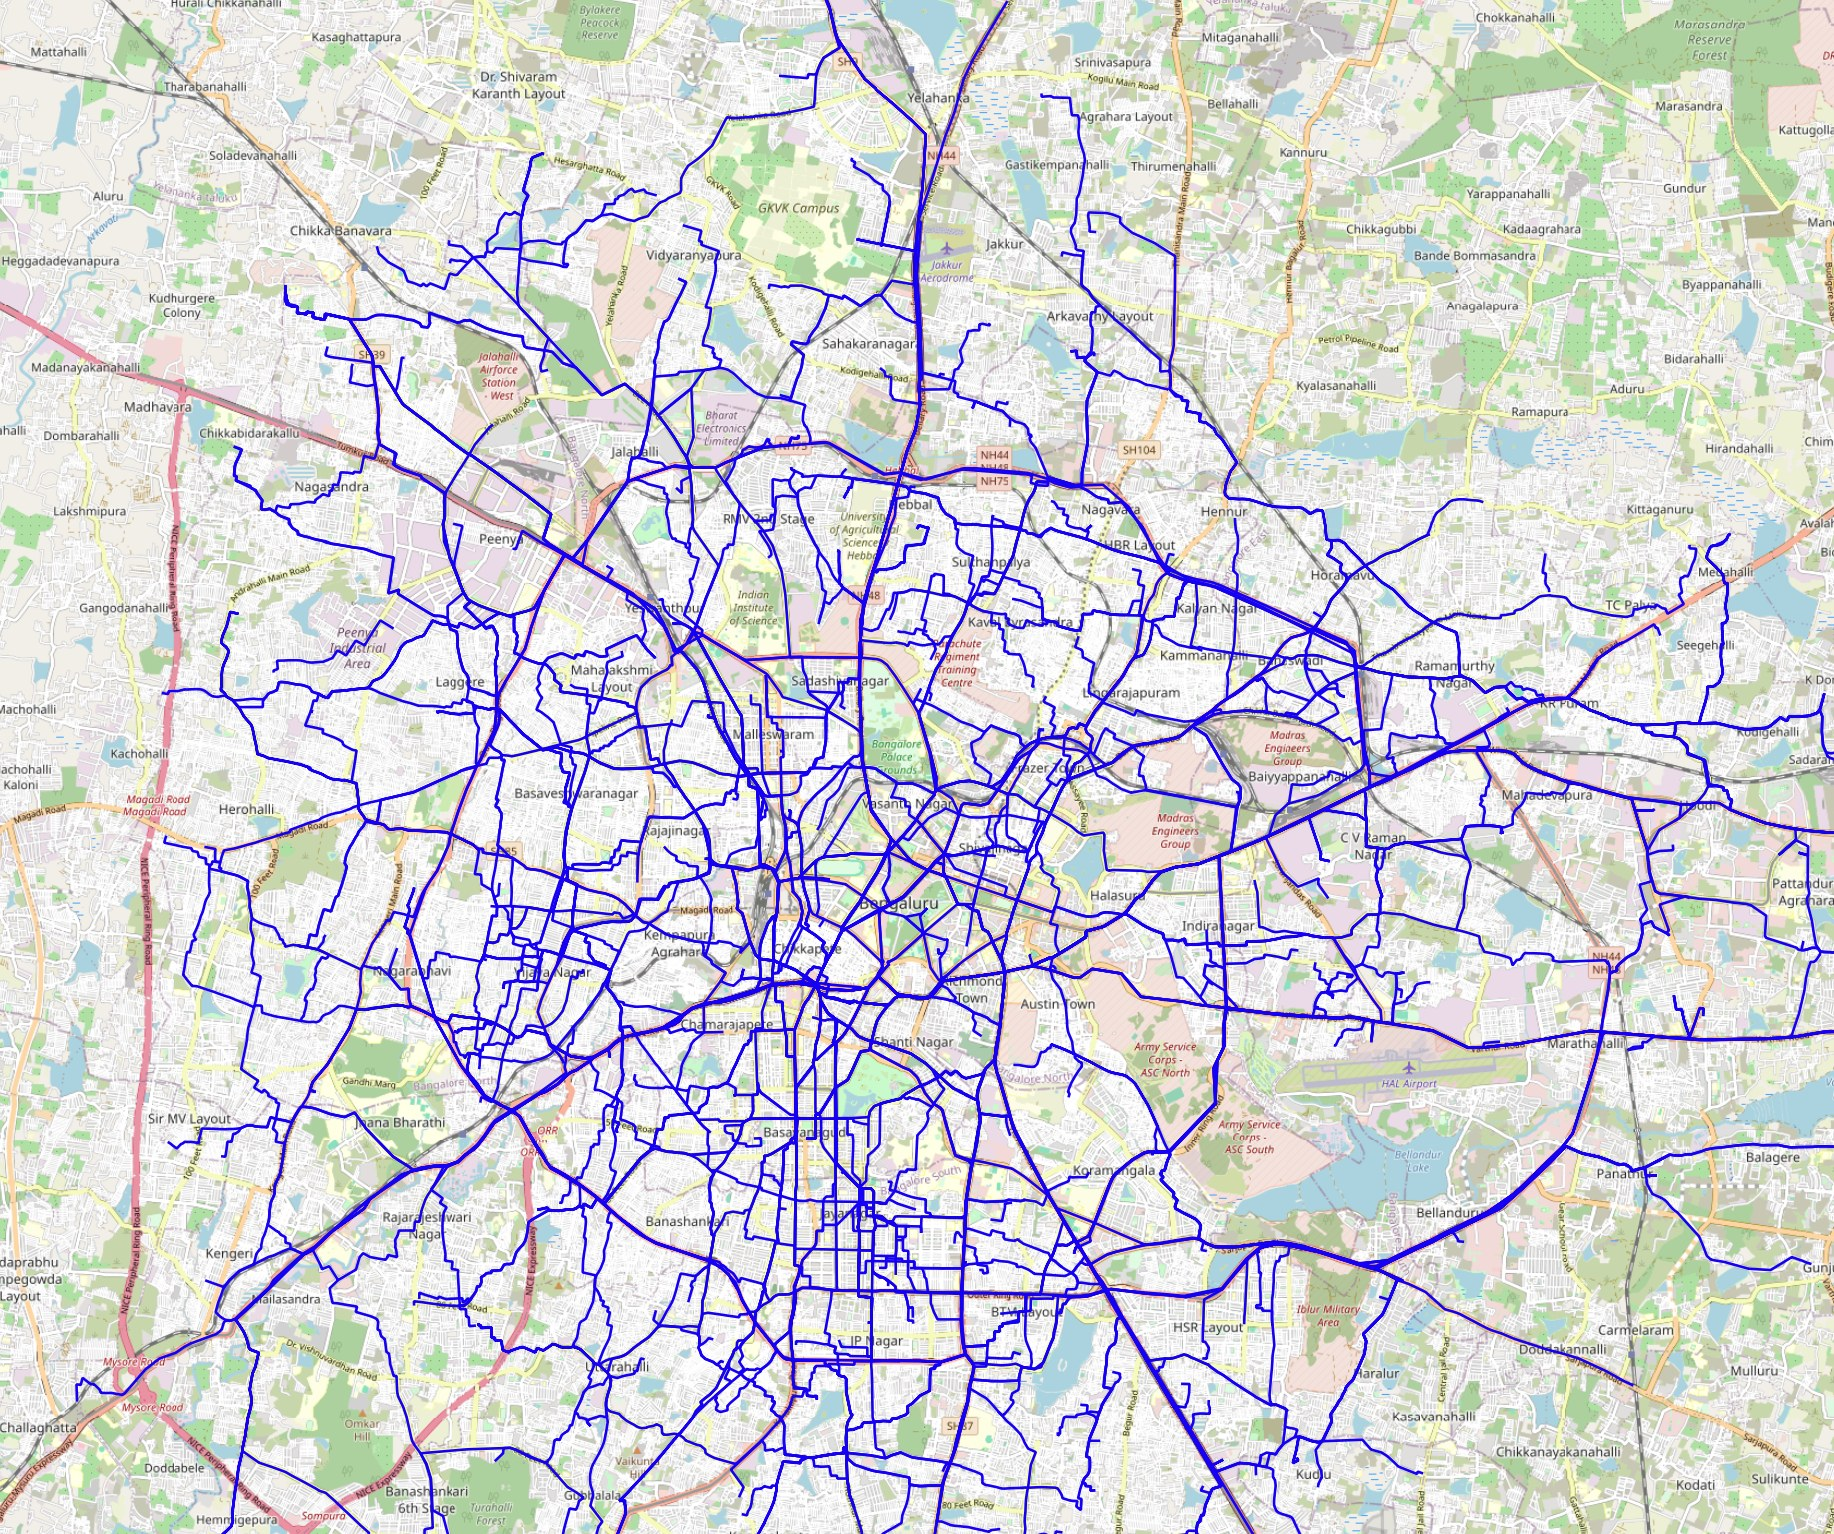
\includegraphics[height=3.4cm]{figures/fig_routes_subarterial.jpg}
\caption{Arterial (left) and sub-arterial (right) routes drawn in QGIS as shortest paths on OpenStreetMap, before overlapping routes were removed. Base map \copyright{} OpenStreetMap contributors.}
\label{fig:route_geometries}
\end{figure}

We sent all 273 routes to the Google Routes API every two hours for seven days, giving 84 snapshots; the analysis below uses the 44 snapshots taken between 1 and 5 April 2026. The places between a route's ends were sent as stops, so Google returned each stretch between two stops as a separate \emph{leg} with its own travel time. Google gives the travel time with traffic only per leg, so the leg is our smallest unit: we treat each leg as a fixed sensor read every two hours. No departure time was set, so each reading is Google's estimate at the moment of the request. Google also returns a traffic state (normal, slow or jam) along the route line, but these states are tied to positions on a line that shifts between queries, so we used them only to animate routes in QGIS and not to measure congestion.

An ETL (extract, transform, load) pipeline turns the raw responses, gigabytes of nested JSON, into tables. It streams one file at a time with Python generators instead of loading everything into memory, and identifies each leg by \emph{spatial hashing}: the leg's end points, rounded to four decimal places, are hashed with MD5, which gives a stable ID even when Google returns slightly different coordinates. The output is a master index with one row per leg and a time-series table with one row per leg per query. Of 689 legs, we removed 125 that lie outside the city, are more than twice as long as the straight line between their ends (both signs of geocoding errors), or are missing from many queries, leaving 564.

\subsection{What the Traffic Data Shows}\label{sec:traffic_findings}
To compare legs of different length, we divide each reading by the median travel time of the same leg, the \emph{relative travel time}, and measure a leg's \emph{variation} as the standard deviation of its travel time divided by its mean. We do not treat the field Google calls the \emph{static duration} as an empty-road time, although our first analysis did. Of all readings, 63\,\% are faster than it; between 02:00 and 04:00 the median reading takes only 0.70 of it; and for 91\,\% of legs the median reading is faster (Fig.~\ref{fig:traffic_by_hour}b). It is also almost fixed for each leg, with no pattern across the day. This fits Google's description of the field as an estimate from historical traffic only, so we do not use delays or congestion ratios built on it.

\begin{figure}[!htb]
\centering
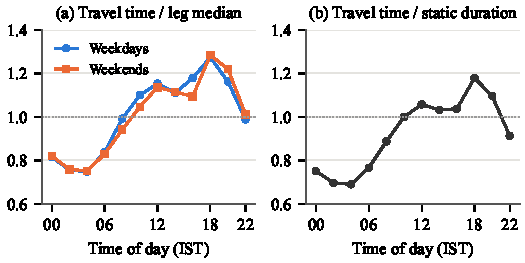
\includegraphics[width=\linewidth]{figures/fig_traffic_by_hour.pdf}
\caption{Median relative travel time by query time (a), and median travel time divided by Google's static duration (b). The dotted line marks 1.}
\label{fig:traffic_by_hour}
\end{figure}

Roads are fastest between 02:00 and 04:00, at about 0.75 of their usual time. Travel time rises through the morning without a sharp peak, stays 10--18\,\% above usual from 10:00 to 16:00 and peaks at 18:00, about 28\,\% above usual (Fig.~\ref{fig:traffic_by_hour}a). For the median leg, the time of day explains 87\,\% of its variation. Legs whose slowest query time is much slower than their fastest, a large \emph{daily swing}, also vary more around their daily pattern (rank correlation 0.55, Fig.~\ref{fig:leg_variation}b). So the busiest legs are somewhat less predictable, but most of what looks like unpredictability is the daily cycle.

We call the fifth of legs with the highest variation, 0.28 or more (113 legs), the \emph{variable legs}. They lie mainly in the centre and along a few radial corridors (Fig.~\ref{fig:legs_map}), and the benchmark uses them to tag its routes (Section~\ref{sec:routes}). At the other end, 21 short legs (4\,\%) reported exactly the static duration in every reading, the bar at zero in Fig.~\ref{fig:leg_variation}a. One possibility is that Google has too little live data for these roads, but we could not check this. Finally, the median speed at each time of day gives the simple baseline of Section~\ref{sec:baseline}.

\begin{figure}[!htb]
\centering
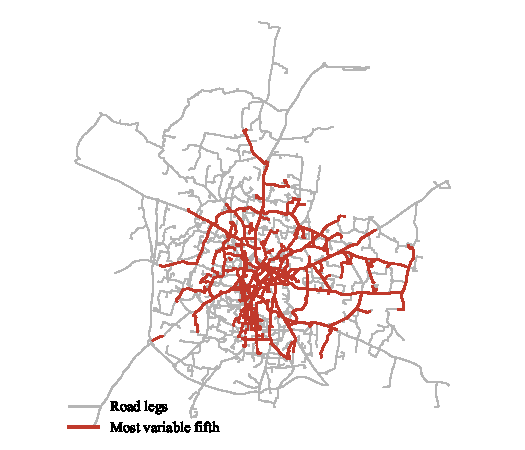
\includegraphics[width=0.7\linewidth,trim=0 0 0 43pt,clip]{figures/fig_legs_map.pdf}
\caption{The 564 road legs used in the analysis. Red: the variable legs, the fifth with the highest variation.}
\label{fig:legs_map}
\end{figure}

\begin{figure}[!htb]
\centering
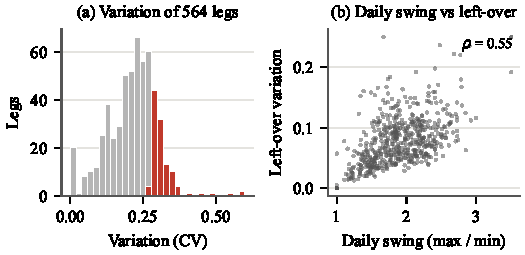
\includegraphics[width=\linewidth]{figures/fig_leg_variation.pdf}
\caption{(a) Variation of the 564 legs; red: the variable legs. (b) Each leg's daily swing against the variation left over after removing the daily pattern.}
\label{fig:leg_variation}
\end{figure}

% The animation figure was removed to shorten this section. To restore it, add:
% \begin{figure}[!htb]\centering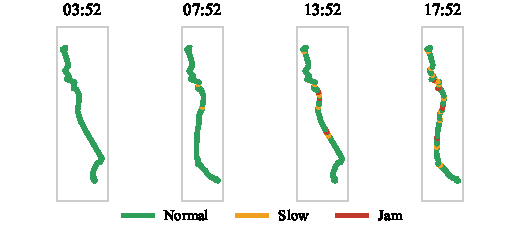
\includegraphics[width=0.8\linewidth]{figures/fig_animation_frames.pdf}
% \caption{Traffic state along Church Road at four times on one weekday.}\label{fig:animation}\end{figure}

\subsection{Reference Answers for the Benchmark}\label{sec:reference}
For the benchmark, Google Maps answers the same 2,016 queries as the LLMs, each a trip between two landmarks at one time on one day (Section~\ref{sec:routes}). Google receives each landmark's coordinates and a departure time in the week of Saturday 28 November to Friday 4 December 2026, with the most thorough traffic-aware routing mode (\texttt{TRAFFIC\_AWARE\_OPTIMAL}) and Google's default \emph{best guess} traffic model. Because these departure times lie in the future, the answers are Google's \emph{predicted} travel times, not measured ones. Google's first suggested route is the reference, and we checked that its start and end points lie close to our landmark coordinates.

Google again gives the time with traffic only for a whole leg. To get road-by-road reference times, a second request for each query adds a stop at every point where the road changes along that query's own route. Stretches shorter than 300~m were merged with a neighbour, a route has at most 11 parts, and every query was checked that its parts add up to the whole route.

% ======================================================================
\section{Benchmark Design}\label{sec:design}

The benchmark turns the research question into a fair test. It fixes which trips are asked about, what each LLM is told, the form its answer must take and how answers are scored against Google Maps. Google and the LLMs receive the same trips at the same days and times, so that differences between their answers come from what the models know rather than from the setup.

\subsection{From a Pilot to Landmarks}
A first pilot used 14 road legs from the traffic data as trips. Most were shorter than 1.5~km and were named by turning coordinates back into addresses (``Start of X''), which an LLM cannot recognise. We therefore built the benchmark on well-known landmarks, which an LLM can know by name. We listed 70 places across the city: metro stations, junctions, bus and railway stations, hospitals, tech parks, malls and campuses. Each was looked up once with Google Places and flagged if its name did not match, it was far from the expected area, another place had the same name, it was an area rather than a point, or it lay more than 150~m from a drivable road. After a manual review, 66 landmarks remained, and 64 of them are used in routes.

\subsection{Routes and Queries}\label{sec:routes}
A \emph{route} is a trip from one landmark to another. Candidate routes were landmark pairs 0.7 to 22~km apart in a straight line. Each was given three tags from its shortest path on OpenStreetMap: a length band (1--5, 5--12 or 12--25~km), a road type from the share of its length on main roads (arterial if at least 0.6, sub-arterial if at most 0.4, otherwise mixed), and its \emph{exposure}, the share of its length on the variable legs of Section~\ref{sec:traffic_findings} (high or low, split at the median of its length band). We chose four routes for each of the 18 combinations, giving 72 routes (Fig.~\ref{fig:routes_map}). No landmark is used more than three times.

A \emph{query} is one route at one time on one day: 08:00, 14:00, 18:00 or 23:00 on each of the seven days, so 28 queries per route and 2,016 in all.

\begin{figure}[!htb]
\centering
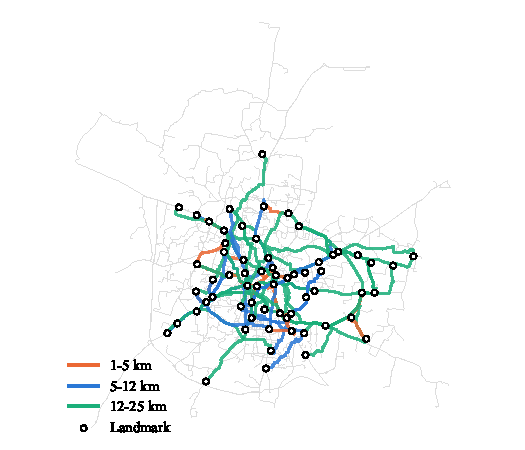
\includegraphics[width=0.8\linewidth,trim=0 0 0 43pt,clip]{figures/fig_routes_map.pdf}
\caption{The 72 benchmark routes as planned (shortest paths on OpenStreetMap), by length band, over the road legs of Section~\ref{sec:traffic_findings}.}
\label{fig:routes_map}
\end{figure}

\subsection{LLM Setup}
Each LLM receives the landmark names, the weekday and the clock time, and nothing else (Table~\ref{tab:setup}). Every query is a separate request with no chat history and no tools. Queries are sent in a fixed shuffled order, so that any change in the model during a run is spread over all routes. Ten routes are asked twice more to measure how much answers change on repeat.

\begin{table}[!htb]
\caption{Setup of the Three Sources}
\label{tab:setup}
\centering
\setlength{\tabcolsep}{3pt}
\begin{tabular}{L{1.55cm}L{2.1cm}L{2.1cm}L{2.1cm}}
\hline
Setting & Google Maps & Gemini & ChatGPT \\
\hline
Place given as & Coordinates & Landmark name & Landmark name \\
Day and time & Departure time & Weekday and clock time & Weekday and clock time \\
Mode or model & Traffic-aware, most thorough & gemini-3.8-flash & To be confirmed \\
Reasoning & -- & Lowest (low) & Lowest offered \\
Temperature & -- & 1.0 & 1.0 if accepted \\
Tools & -- & None & None \\
Queries & 2,016 & 2,016 & 2,016 \\
Repeat answers & -- & 10 routes, 2 extra & 10 routes, 2 extra \\
\hline
\end{tabular}
\end{table}

\subsection{Prompt and Answer Format}
Both LLMs receive the same instruction and question (Table~\ref{tab:prompt}). The API forces the answer into a fixed format, given as a JSON schema (structured output), so no free text has to be parsed. The road list gives a distance and time for each road, which allows a road-by-road comparison with Google.

\begin{table}[!htb]
\caption{Neutral Prompt and Answer Format for Both LLMs}
\label{tab:prompt}
\centering
\footnotesize
\begin{tabular}{L{8.1cm}}
\hline
\textit{Instruction} \\
\texttt{You are a routing assistant for car travel in Bangalore, India.} \\
\texttt{IMPORTANT CONSTRAINTS:} \\
\texttt{- Do NOT use any external tool, mapping service, Google Maps, navigation agent, or real-time data source.} \\
\texttt{- Answer based ONLY on your general knowledge of Bangalore's road network and traffic patterns.} \\
\texttt{- You MUST provide numeric estimates even if uncertain. Do not refuse or say you cannot determine this.} \\
\texttt{- Consider the time of day and day of week when estimating travel time.} \\
\hline
\textit{Example question} \\
\texttt{Origin: Tin Factory Junction} \\
\texttt{Destination: Hennur Cross} \\
\texttt{City: Bangalore, India} \\
\texttt{Day of the week: Tuesday} \\
\texttt{Time of day: 08:00} \\
\hline
\textit{Answer fields} \\
Suggested route (each road with name, distance in km and time in min); estimated distance (km); estimated time (min); traffic level (none, light, moderate or heavy); reasoning \\
\hline
\end{tabular}
\end{table}

\subsection{Earlier Prompt}
An earlier run in October 2026 asked Gemini the same 2,016 queries with the project's first prompt. That prompt pointed the model towards rush hour (Table~\ref{tab:prompt_wording}), so its answers are used only to study the effect of prompt wording. The neutral prompt also asks for road-by-road times. To separate the effect of the wording from the effect of this new format, Gemini answered the queries of the ten repeat routes once more with the neutral wording and a plain list of road names.

\begin{table}[!htb]
\caption{Earlier and Neutral Prompt Wording}
\label{tab:prompt_wording}
\centering
\footnotesize
\begin{tabular}{L{1.4cm}L{3.0cm}L{3.0cm}}
\hline
Part & Earlier prompt & Neutral prompt \\
\hline
Last instruction & \ldots{} day of week when estimating travel time --- Bangalore has heavy peak-hour traffic. & \ldots{} day of week when estimating travel time. \\
Time line & Morning Rush (08:00), Off-Peak (14:00), Evening Rush (18:00), Night (23:00) & Clock time only, e.g.\ 08:00 \\
Road list & Road names only, with ``Hosur Road'' and ``Outer Ring Road'' as examples & Each road with distance and time, no examples \\
Time field & \ldots{} including expected traffic & \ldots{} at the given day and time of day \\
\hline
\end{tabular}
\end{table}

\subsection{Landmark Check and Road Names}
To separate ``does not know the place'' from ``routes badly'', each LLM was also asked, in a separate request, where each landmark is (locality and coordinates). A landmark counts as \emph{misplaced} if the LLM's point is more than 2~km from Google's and the locality does not match.

To compare roads, Google's route line was \emph{map-matched} to OpenStreetMap: a point every 20~m was matched to the nearest road within 25~m, and a road name was kept if it held for at least three points. Road names from Google's turn-by-turn instructions were added. LLM road names were cleaned (case, abbreviations such as ``Rd'' and ``ORR'') and counted as the same road as a reference name when their token-set similarity score, a fuzzy string match that ignores word order, was at least 85 out of 100. The \emph{reference list} joins OpenStreetMap names, Google's instruction names and the BBMP road list.

\subsection{Measures and Statistics}
Table~\ref{tab:measures} defines the measures. Our main error measure is the \emph{typical miss}, the median percentage error: an LLM value 25\,\% above or 25\,\% below Google's both count as a 25\,\% miss. The 28 queries of one route are not independent, so 95\,\% confidence intervals come from resampling whole routes 2,000 times (a route-level bootstrap), and group differences are tested by shuffling group labels 5,000 times on per-route values (a permutation test). Gemini and ChatGPT are compared on the same queries. Because route length differs between road types, road-type comparisons are repeated on routes of 5~km or more.

\begin{table}[!htb]
\caption{Benchmark Measures}
\label{tab:measures}
\centering
\footnotesize
\begin{tabular}{L{1.8cm}L{2.8cm}L{2.9cm}}
\hline
Measure & Definition & Meaning \\
\hline
Ratio to Google & LLM value / Google value & Above 1: LLM too high \\
Typical miss & Median of $|\text{LLM}/\text{Google}-1|$ & Size of the miss, ignoring direction; 0 is perfect \\
Traffic index & Google time / route's fastest of its 28 times & 1 is the route's best case \\
Rush-hour multiplier & Mean of 08:00 and 18:00 / 23:00, weekdays & How much slower rush hour is than night \\
Rank correlation & Spearman's $\rho$ & $-1$ to 1: do two series rise and fall together \\
Road validity & Share of named roads found in the reference list & 0 to 1 \\
Road overlap & Shared roads / roads in either list (Jaccard index) & 0 to 1 \\
Repeat spread & Coefficient of variation over three answers & 0: identical answers \\
\hline
\end{tabular}
\end{table}

\subsection{Simple Formula Baseline}\label{sec:baseline}
As a rule of thumb, we estimate distance as the straight-line distance times 1.22, the median ratio of road to straight-line distance (the \emph{detour factor}) among the candidate routes, and time as that distance divided by the median speed of the traffic data (Section~\ref{sec:traffic_findings}) near the same time of day, separately for weekdays and weekends. The formula knows the exact coordinates, which the LLMs do not, and its speeds come from a few days of data.

% ======================================================================
\section{Results}\label{sec:results}
% ChatGPT has not been run yet. When its answers exist, add a ChatGPT column to each table
% and a ChatGPT series to each figure, and rename the subsections back to "the LLMs".
This section answers the five questions of Section~I in turn. It first describes Google's reference answers, then Gemini's knowledge of places and roads, its distances and times, its sense of traffic over the day, the trips where it does worst, and the effect of the prompt. ChatGPT has not been run yet, so the results are for Gemini; Google Maps is the reference throughout.

\subsection{Google Maps Reference}
All 2,016 Google requests succeeded, and every start and end point lay within the allowed distance of its landmark. Table~\ref{tab:route_groups} shows the 72 routes by length and road type. Google's predicted traffic follows a clear weekly pattern (Fig.~\ref{fig:google_heatmap}). On weekdays, the median route is 19\,\% above its fastest time at 08:00, 35\,\% at 14:00, 63\,\% at 18:00 and 5\,\% at 23:00. Weekends are lighter in the morning and evening, and on Sunday morning routes are almost at their fastest. Google used more than one path during the week on 37 of the 72 routes.

\begin{figure}[!htb]
\centering
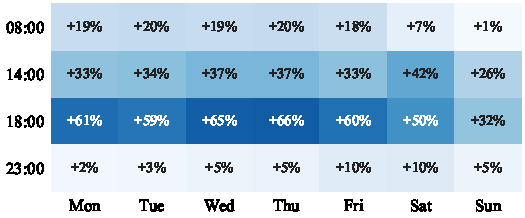
\includegraphics[width=\linewidth]{figures/fig_google_heatmap.pdf}
\caption{Google's predicted traffic for the benchmark week: median traffic index of the 72 routes, shown as the percentage above each route's fastest time.}
\label{fig:google_heatmap}
\end{figure}

\begin{table}[!htb]
\caption{Routes by Length and Road Type}
\label{tab:route_groups}
\centering
\begin{tabular}{lcccc}
\hline
Route length & Arterial & Mixed & Sub-arterial & Total \\
\hline
1--5~km & 7 & 4 & 6 & 17 \\
5--12~km & 16 & 7 & 4 & 27 \\
12~km or more & 21 & 5 & 2 & 28 \\
Total & 44 & 16 & 12 & 72 \\
\hline
\end{tabular}
\end{table}

\subsection{Gemini against Google Maps}

\subsubsection{Places and Road Names}
Gemini placed all 64 landmarks within 2~km of Google's point, with a median distance of 0.25~km, so none counts as misplaced (Fig.~\ref{fig:landmark_error}, Table~\ref{tab:checks}). The landmark check was run once, in October; its prompt contains no traffic wording. Across all answers Gemini named 2,069 distinct roads, and 92\,\% of them match a reference name; within one answer, 96\,\% of the named roads match on average. Matching is lower on routes along smaller roads (91\,\% against 97\,\% on main roads).

\begin{table}[!htb]
\caption{Place, Road Name and Repeat Answer Checks}
\label{tab:checks}
\centering
\begin{tabular}{L{5.2cm}c}
\hline
Measure & Gemini \\
\hline
Landmarks misplaced & 0 of 64 \\
Median landmark error & 0.25~km \\
Distinct road names found in the reference list & 92\,\% \\
Repeat spread, distance & 3.9\,\% \\
Repeat spread, time & 5.8\,\% \\
Same traffic level on repeat & 93\,\% \\
Road-list overlap between repeats & 0.43 \\
\hline
\end{tabular}
\end{table}

\begin{figure}[!htb]
\centering
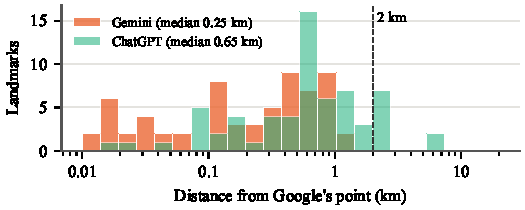
\includegraphics[width=\linewidth]{figures/fig_landmark_error.pdf}
\caption{Distance between Gemini's point and Google's point for each of the 64 landmarks. The dashed line marks the 2~km limit of the landmark check.}
\label{fig:landmark_error}
\end{figure}

\subsubsection{Distance and Time}
Table~\ref{tab:accuracy} summarises accuracy over all 2,016 queries. Gemini's distances are slightly long (median ratio 1.08, longer than Google's in 67\,\% of queries), with a typical miss of 14\,\%. Its times have a median ratio of 1.01 but a typical miss of 23\,\%, and only 23\,\% of times fall within 10\,\% of Google's. In absolute terms the typical miss is 1.3~km and 6.1~minutes. In Fig.~\ref{fig:scatter}, distances follow the line of equal values, while times split by the time of day: rush-hour answers lie above the line and night answers below it. Table~\ref{tab:worked_example} shows one route. At 08:00 Gemini's time is close to Google's, but at 23:00 it gives 9 minutes against Google's 19, and it names only one of the main roads on Google's path.

\begin{table}[!htb]
\caption{Distance and Time Accuracy}
\label{tab:accuracy}
\centering
\setlength{\tabcolsep}{4pt}
\begin{tabular}{lcccccc}
\hline
 & \multicolumn{3}{c}{Distance} & \multicolumn{3}{c}{Time} \\
\cline{2-4}\cline{5-7}
Source & Ratio & Miss & ${\le}10\,\%$ & Ratio & Miss & ${\le}10\,\%$ \\
\hline
Gemini & 1.08 & 14\,\% & 35\,\% & 1.01 & 23\,\% & 23\,\% \\
Simple formula & 0.92 & 10\,\% & -- & 0.90 & 16\,\% & -- \\
\hline
\multicolumn{7}{p{7.6cm}}{\footnotesize Ratio: median of LLM / Google. ${\le}10\,\%$: share of queries within 10\,\% of Google.}
\end{tabular}
\end{table}

\begin{figure}[!htb]
\centering
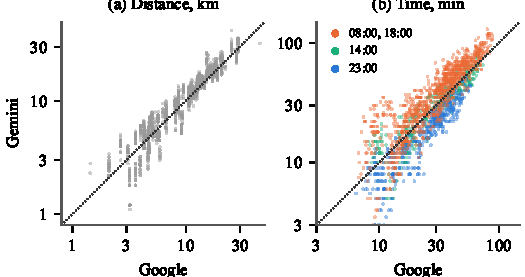
\includegraphics[width=\linewidth]{figures/fig_scatter.pdf}
\caption{Gemini against Google Maps for all 2,016 queries, on log axes: (a) distance, (b) travel time by query time. The dotted line marks equal values.}
\label{fig:scatter}
\end{figure}

\begin{table}[!htb]
\caption{Worked Example: Tin Factory Junction to Hennur Cross, Tuesday 1 December}
\label{tab:worked_example}
\centering
\setlength{\tabcolsep}{3pt}
\footnotesize
\begin{tabular}{L{1.15cm}ccL{1.3cm}L{3.3cm}}
\hline
Source & km & min & Traffic & Main roads named \\
\hline
\multicolumn{5}{l}{\textit{08:00}} \\
Google & 8.1 & 21.3 & +45\,\% & Outer Ring Road, NH 44, Hennur Bagalur Main Rd \\
Gemini & 7.5 & 24.0 & Moderate & Old Madras Road, Outer Ring Road \\
\multicolumn{5}{l}{\textit{23:00}} \\
Google & 8.1 & 18.8 & +28\,\% & Same as at 08:00 \\
Gemini & 6.4 & 9.0 & Light & Outer Ring Road, Hennur Bagalur Main Road \\
\hline
\multicolumn{5}{l}{\footnotesize Google's traffic is its traffic index, the time above the route's fastest.}
\end{tabular}
\end{table}

\subsubsection{Time of Day}
Table~\ref{tab:time_ratio} gives Gemini's time ratio to Google at each query time. On weekdays Gemini is 29\,\% too slow at 08:00, 32\,\% too slow at 18:00 and 25\,\% too fast at 23:00; only the 14:00 answers are close. Fig.~\ref{fig:day_shape} shows why: relative to the same trip at weekday 23:00, Gemini makes trips 2.03 times longer at 08:00 and 2.75 times longer at 18:00, while Google predicts 1.13 and 1.52. Each route's rush-hour multiplier is larger for Gemini than for Google, on all 72 routes (Fig.~\ref{fig:multiplier}); the medians are 2.40 and 1.34, and the two hardly agree on which routes are worst (rank correlation 0.11). The gap is largest for short trips (1--5~km: 2.61 against 1.24). One route reverses Google's pattern: from Yeshwanthpur Metro to Peenya Metro, Google predicts 21 minutes at weekday 23:00 and 16 at 08:00, while Gemini gives 8 and 15.

Gemini's traffic labels follow the clock (Fig.~\ref{fig:traffic_levels}). On weekdays, every 14:00 answer is ``moderate'', every 18:00 answer ``heavy'' and every 23:00 answer ``light''; at 08:00, 56\,\% are ``heavy''. Even so, the labels rise and fall with Google's traffic index (rank correlation 0.73), and within a route the order of Gemini's 28 times agrees with Google's (median rank correlation 0.81).

\begin{table}[!htb]
\caption{Time Ratio to Google by Time of Day}
\label{tab:time_ratio}
\centering
\begin{tabular}{lcccc}
\hline
Source & 08:00 & 14:00 & 18:00 & 23:00 \\
\hline
Gemini, weekday & 1.29 & 0.98 & 1.32 & 0.75 \\
Gemini, weekend & 0.92 & 0.92 & 1.13 & 0.72 \\
Simple formula, weekday & 0.90 & 0.90 & 0.86 & 0.89 \\
\hline
\end{tabular}
\end{table}

\begin{figure}[!htb]
\centering
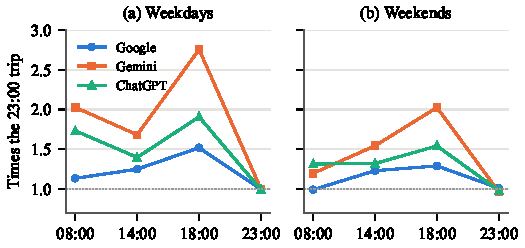
\includegraphics[width=\linewidth]{figures/fig_day_shape.pdf}
\caption{Shape of the day: median travel time at each query time divided by the same route at weekday 23:00, for Google and Gemini.}
\label{fig:day_shape}
\end{figure}

\begin{figure}[!htb]
\centering
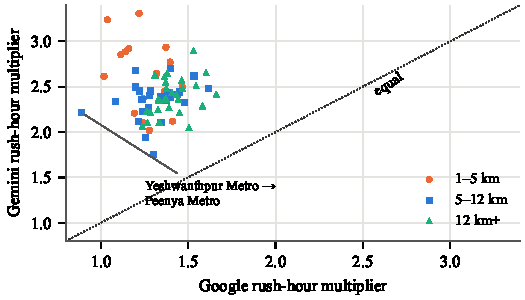
\includegraphics[width=\linewidth]{figures/fig_multiplier.pdf}
\caption{Rush-hour multiplier of each route: Gemini against Google, by route length. Every route lies above the dotted line of equal values.}
\label{fig:multiplier}
\end{figure}

\begin{figure}[!htb]
\centering
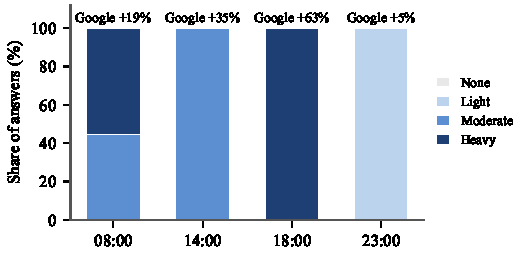
\includegraphics[width=\linewidth]{figures/fig_traffic_levels.pdf}
\caption{Traffic levels reported by Gemini at each weekday query time, with Google's median traffic index above each bar.}
\label{fig:traffic_levels}
\end{figure}

\subsubsection{Road Choice}
Of the roads Gemini names, 60\,\% are on Google's route (precision), but it names only 20\,\% of Google's roads (recall), and the overlap of the two lists is 0.17 (Table~\ref{tab:road_overlap}). All three fall on routes along smaller roads. Gemini names a median of four roads per answer, while Google's route has a median of six. In the road-by-road comparison, 90\,\% of queries have at least one road that pairs with a Google sub-route, with 1.7 pairs per query covering a median of 37\,\% of Google's route length. On these roads Gemini's distances and times are about 20\,\% too high, with a typical miss of 48\,\% for distance and 47\,\% for time, although its road values always add up to its own totals. The time-of-day pattern repeats at road level: the paired-road time ratio is 1.28 at 08:00, 1.13 at 14:00, 1.49 at 18:00 and 0.89 at 23:00.

Fig.~\ref{fig:paths} draws two trips. On the first, Gemini names the Outer Ring Road, which carries most of Google's path, yet the overlap score is only 0.09 because Google's route lists many short named stretches; a low overlap can therefore hide a sensible route. On the second, Gemini gives the direct 1.2~km along Mahatma Gandhi Road, while Google's path loops north for 3.2~km, possibly because of one-way streets around Trinity Circle.

\begin{figure}[!htb]
\centering
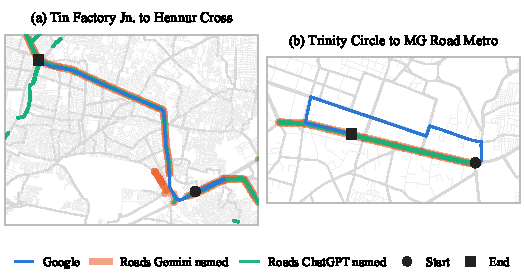
\includegraphics[width=\linewidth]{figures/fig_paths.pdf}
\caption{Google's path and the roads Gemini named for two queries on Tuesday at 08:00. Gemini gives road names, not coordinates, so its roads are drawn as the OpenStreetMap roads near the trip whose names match (score of 85 or more). Map data \copyright{} OpenStreetMap contributors.}
\label{fig:paths}
\end{figure}

\begin{table}[!htb]
\caption{Road Overlap with Google by Road Type}
\label{tab:road_overlap}
\centering
\begin{tabular}{lccc}
\hline
Road type & Overlap & Recall & Precision \\
\hline
Arterial & 0.18 & 0.21 & 0.64 \\
Mixed & 0.19 & 0.21 & 0.66 \\
Sub-arterial & 0.11 & 0.14 & 0.39 \\
All routes & 0.17 & 0.20 & 0.60 \\
\hline
\end{tabular}
\end{table}

\subsubsection{Repeat Answers}
The 280 queries of the ten repeat routes were each answered three times. Distances vary by 3.9\,\% and times by 5.8\,\% between answers, the traffic level is the same in 93\,\% of queries, and the road lists of two answers overlap by 0.43 on average (Table~\ref{tab:checks}). Gemini's errors are therefore mostly repeated, not random.

\subsubsection{Simple Formula}
The simple formula misses Google by 16\,\% in time and 10\,\% in distance (Table~\ref{tab:accuracy}), and its times are about 10\,\% too fast at every time of day. Gemini beats it on 43\,\% of queries for time and 46\,\% for distance. Only at 14:00 is Gemini better, with a typical time miss of 14\,\% against 16\,\%, winning on 59\,\% of queries; at the other three times it wins on 32 to 41\,\%.

\subsection{Where Gemini Does Worst}
Table~\ref{tab:group_tests} compares route groups using each route's typical miss, and Fig.~\ref{fig:where_worst} shows the main ones. Length matters most: short routes have about one and a half times the time miss and nearly three times the distance miss of long routes. Routes along smaller roads look worse on both measures, but half of them are short. On routes of 5~km or more, smaller roads still have twice the distance miss, but the same time miss. Exposure to the variable legs makes no difference. Table~\ref{tab:outliers} lists the routes with the largest misses and the closest one.

\begin{figure}[!htb]
\centering
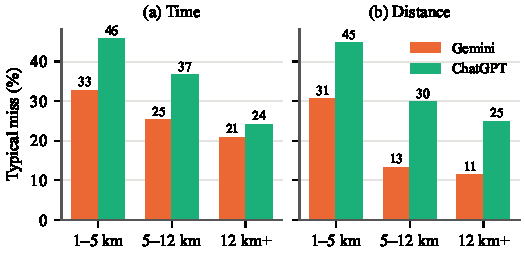
\includegraphics[width=\linewidth]{figures/fig_where_worst.pdf}
\caption{Gemini's typical miss (median percentage error per route) by route length (a), and on main and smaller roads for routes of 5~km or more (b).}
\label{fig:where_worst}
\end{figure}

\begin{table}[!htb]
\caption{Comparisons between Route Groups (Typical Miss per Route)}
\label{tab:group_tests}
\centering
\setlength{\tabcolsep}{3pt}
\footnotesize
\begin{tabular}{L{3.5cm}lccc}
\hline
Groups A and B & Measure & A & B & $p$ \\
\hline
Short vs long (17, 28) & Time & 33\,\% & 21\,\% & 0.0002 \\
 & Distance & 31\,\% & 11\,\% & 0.0002 \\
Main vs smaller (44, 12) & Time & 22\,\% & 26\,\% & 0.05 \\
 & Distance & 12\,\% & 31\,\% & 0.0008 \\
Same, 5~km+ (37, 6) & Time & 21\,\% & 22\,\% & 0.59 \\
 & Distance & 11\,\% & 23\,\% & 0.006 \\
High vs low exposure (49, 23) & Time & 23\,\% & 22\,\% & 1.0 \\
 & Distance & 13\,\% & 17\,\% & 0.19 \\
\hline
\multicolumn{5}{p{7.4cm}}{\footnotesize Short: 1--5~km; long: 12~km or more. Number of routes in brackets. $p$: permutation test, 5,000 shuffles.}
\end{tabular}
\end{table}

\begin{table}[!htb]
\caption{Outlier Routes (Median over 28 Queries Unless Stated)}
\label{tab:outliers}
\centering
\setlength{\tabcolsep}{3pt}
\footnotesize
\begin{tabular}{L{2.4cm}C{1.05cm}C{1.05cm}L{2.6cm}}
\hline
Route & Google & Gemini & Possible reason \\
\hline
Esteem Mall Hebbal to Manyata Tech Park & 4.0~km, 9~min & 5.5~km, 16~min & Reputation of the Hebbal area for traffic \\
Trinity Circle to MG Road Metro & 3.2~km, 12~min & 1.2~km, 5~min & One-way streets lengthen Google's path \\
KR Puram Railway Station to Phoenix Marketcity & 2.7~km, 9~min & 4.2~km, 14~min & Gemini takes a longer path; unclear \\
Yeshwanthpur Metro to Peenya Metro, weekday 23:00 & 21~min & 8~min & Heavy goods traffic at night \\
\textit{Closest:} Shivajinagar Bus Station to Mekhri Circle & 5.1~km, 15~min & 5.2~km, 17~min & -- \\
\hline
\end{tabular}
\end{table}

\subsection{Effect of Prompt Wording}
Over all 72 routes, the earlier prompt made Gemini call 92\,\% of weekday 08:00 queries ``heavy'', against 56\,\% with the neutral prompt, and gave a typical 08:00 time of 45 instead of 40~minutes. For the same query, the neutral answer is a median of 0.91 times the earlier one. Distances hardly change (11.5 against 11.2~km). Table~\ref{tab:prompt_effect} separates wording from answer format on the ten repeat routes. Changing only the wording lowers the 08:00 time from 45 to 39~minutes and the share of ``heavy'' from 98\,\% to 60\,\%, but leaves the rush-hour multiplier near 2 and every 18:00 answer ``heavy''. Asking for road-by-road times then raises the multiplier from 1.96 to 2.37 and shortens night trips (Fig.~\ref{fig:prompt_effect}). Google's multiplier for these routes is 1.32.

\begin{table}[!htb]
\caption{Gemini with Three Prompt Versions on the Ten Repeat Routes (Weekdays)}
\label{tab:prompt_effect}
\centering
\setlength{\tabcolsep}{3pt}
\footnotesize
\begin{tabular}{L{2.5cm}cccc}
\hline
 & Earlier & \multicolumn{2}{c}{Neutral wording} & \\
\cline{3-4}
Measure & prompt & Whole & By road & Google \\
\hline
08:00 time (min) & 45 & 39 & 39 & 30 \\
14:00 time (min) & 35 & 35 & 32 & 35 \\
18:00 time (min) & 55 & 50 & 53 & 39 \\
23:00 time (min) & 22 & 22 & 20 & 29 \\
Rush-hour multiplier & 2.07 & 1.96 & 2.37 & 1.32 \\
08:00 ``heavy'' & 98\,\% & 60\,\% & 60\,\% & -- \\
18:00 ``heavy'' & 100\,\% & 100\,\% & 100\,\% & -- \\
\hline
\end{tabular}
\end{table}

\begin{figure}[!htb]
\centering
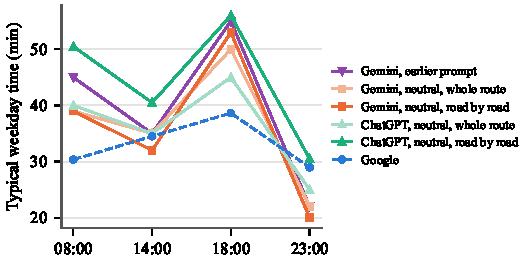
\includegraphics[width=\linewidth]{figures/fig_prompt_effect.pdf}
\caption{Typical weekday travel time on the ten repeat routes for three prompt versions of Gemini, with Google.}
\label{fig:prompt_effect}
\end{figure}

% ======================================================================
\section{Discussion and Limitations}\label{sec:discussion}

The results show what Gemini gets right and wrong. This section asks what they suggest about its knowledge, how they compare with what we expected at the start of the project, what they mean for someone who uses an LLM to plan a trip, and where our conclusions stop.

% ChatGPT results are not in yet. When they arrive, add one sentence per paragraph
% on whether ChatGPT shows the same pattern, and rename the first subsection.
\subsection{What Gemini Knows}
Gemini knows the city's places and road names, but not which roads a driver would take: it places every landmark correctly and names real roads, yet names only a fifth of the roads on Google's route. Its distances are close. Its travel times look accurate on average only because two errors cancel: it is too slow in rush hour and too fast at night. It orders a route's times roughly as Google does, because both put 18:00 slowest and 23:00 fastest, but it adds about the same rush-hour penalty to every route, whether or not Google expects that route to be slow. In short, it knows the clock better than the road. Its repeat answers barely change, so these errors are systematic rather than random.

The largest gap is at 08:00. Google predicts weekday traffic at 08:00 only 13\,\% above night, and the city-wide traffic data (Section~\ref{sec:traffic_findings}) also shows no sharp morning peak. One possibility is that Bangalore's morning peak comes later than 08:00, so a model that treats 08:00 as rush hour is early; we did not ask at other morning times, so this remains untested. On the Yeshwanthpur to Peenya route, where Google predicts night to be slower than 08:00 in both weeks of its data, heavy goods traffic near the Peenya industrial area is one possible reason.

The road-by-road answers show that a good total does not mean good parts: errors on single roads cancel in the sum. A possible reading is that Gemini starts from a sense of the whole trip and splits it over roads, rather than adding up roads it knows; our data cannot tell these apart. Short trips are hardest; one possibility is that an error of a few minutes or a kilometre weighs more on a short trip. Main roads help with distance but not with time, and the variable legs make no difference, so Gemini's time errors seem to come from its view of the clock rather than from particular roads.

Prompt wording explains only part of the rush-hour bias. The earlier wording mainly inflated 08:00, but with neutral wording rush hour is still about twice the night time, and asking for road-by-road times raised this ratio further. A study of LLM travel times should therefore report both the wording and the answer format.

\subsection{Earlier Expectations}
At the start of the project we expected travel times to be weaker than distances, and they were (typical miss 23\,\% against 14\,\%). We expected main roads to be easier than side roads; this held for distance but not for time (Table~\ref{tab:group_tests}). Routes through the variable legs were not harder, against our expectation. Two further expectations, that giving the model map context would help and that an India-focused map service would match Google more closely, were not tested.

\subsection{Practical Meaning}
For a traveller, Gemini gives a usable rough distance between well-known places more than 5~km apart. Its weekday travel times should be read as about 30\,\% too long at rush hour and 25\,\% too short at night, its road-by-road figures should not be trusted, and its ``heavy traffic'' label adds little beyond the time already in the question. A simple formula from the exact coordinates does better (Section~\ref{sec:results}).

\subsection{Limitations}
\emph{Reference.} Google's times are predictions for one week, not measured drives, so ``close to Google'' is not the same as ``close to the real trip''. The earlier prompt was compared against a different Google week. Gemini's questions contain no date, so its answers under the two prompts can be compared directly, and Google's own pattern was almost the same in both weeks.

\emph{Models and prompts.} Only Gemini has been tested so far, at one setting (lowest reasoning, temperature 1.0), and results may change with later model versions. The neutral prompt still asks the model to consider the time of day. The earlier and neutral prompts differ in several places at once; the format-control run separates the answer format from the wording, but not the individual wording changes from each other.

\emph{Routes and roads.} Only 12 routes run mainly on smaller roads, and only six of them are 5~km or longer, so road-type results are indicative. Road matching depends on names: Google may call a road ``NH 44'' where others say ``Outer Ring Road'', so validity and overlap are lower bounds, and paired roads cover a median of 37\,\% of Google's route length.

\emph{Traffic data.} The city-wide traffic data covers a short period, its readings are Google's estimates at the moment of each request, and its static duration is not an empty-road time. The simple formula's speeds come from this data, and the formula knows the exact coordinates, which the LLMs do not.

% ======================================================================
\section{Conclusion and Future Work}\label{sec:conclusion}

\subsection{Conclusion}
We asked how close an LLM, using only its own knowledge, can get to Google Maps on routes, distances and travel times in Bangalore. For Gemini, the answer depends on what is asked. It knows where well-known places are and names real roads, but it chooses only a fifth of the roads on Google's route. Its distances are fairly close, with a typical miss of 14\,\%. Its travel times are weaker, with a typical miss of 23\,\%, and their average looks right only because they are too slow in rush hour and too fast at night: Gemini adds a similar rush-hour penalty to every trip, set by the clock rather than by the road. It does worst on short trips, and its road-by-road figures are far less reliable than its totals. Removing rush-hour wording from the prompt reduced the morning bias but did not remove it, and the answer format changed the results as much as the wording. A one-line formula that knows the exact coordinates beat Gemini on both distance and time. Gemini's travel times are therefore a rough guide at best and no substitute for a navigation tool. Along the way, the city-wide traffic data showed that Google's static duration is not an empty-road time, and that most of the variation on Bangalore's main roads follows a daily cycle that peaks at 18:00.

\subsection{Future Work}
The first next step is to run ChatGPT on the same queries. The benchmark can then test whether giving the model map context, such as the roads near a trip, closes the gap, and whether higher reasoning settings help. Asking at more morning times would test whether Bangalore's morning peak comes later than 08:00. More routes on smaller roads would make the road-type comparison firmer, and comparing with MapmyIndia, an India-focused map service, or with measured trip times would show how much of the remaining gap lies in the reference rather than in the model.

% ======================================================================
\section*{Acknowledgment}
Thanks to the supervisor, Prof. Vinayak Naik, and to others who helped.

\section*{Data Availability}
What can be shared, and why raw Google and LLM data is not published.

% References: each was checked to exist; the author should read each one before submission.
\begin{thebibliography}{00}
\bibitem{gurnee2024} W. Gurnee and M. Tegmark, ``Language models represent space and time,'' in \textit{Proc. Int. Conf. Learn. Represent. (ICLR)}, 2024.
\bibitem{bhandari2023} P. Bhandari, A. Anastasopoulos, and D. Pfoser, ``Are large language models geospatially knowledgeable?'' in \textit{Proc. 31st ACM SIGSPATIAL Int. Conf. Adv. Geogr. Inf. Syst.}, 2023.
\bibitem{manvi2024} R. Manvi, S. Khanna, G. Mai, M. Burke, D. Lobell, and S. Ermon, ``GeoLLM: Extracting geospatial knowledge from large language models,'' in \textit{Proc. Int. Conf. Learn. Represent. (ICLR)}, 2024.
\bibitem{roberts2023} J. Roberts \textit{et al.}, ``GPT4GEO: How a language model sees the world's geography,'' arXiv:2306.00020, 2023.
\bibitem{chen2024} W. Chen, M.-W. Su, N. Mehjabin, and M. L. Cummings, ``Can LLMs plan paths in the real world?'' arXiv:2411.17912, 2024.
\bibitem{dihan2025} M. L. Dihan \textit{et al.}, ``MapEval: A map-based evaluation of geo-spatial reasoning in foundation models,'' in \textit{Proc. 42nd Int. Conf. Mach. Learn. (ICML)}, PMLR vol. 267, 2025.
\bibitem{guo2026} H. Guo \textit{et al.}, ``TransitLM: A large-scale dataset and benchmark for map-free transit route generation,'' arXiv:2605.22355, 2026.
\bibitem{akbar2023} P. A. Akbar, V. Couture, G. Duranton, and A. Storeygard, ``Mobility and congestion in urban India,'' \textit{Amer. Econ. Rev.}, vol. 113, no. 4, pp. 1083--1111, 2023.
\bibitem{sclar2024} M. Sclar, Y. Choi, Y. Tsvetkov, and A. Suhr, ``Quantifying language models' sensitivity to spurious features in prompt design or: How I learned to start worrying about prompt formatting,'' in \textit{Proc. Int. Conf. Learn. Represent. (ICLR)}, 2024.
\end{thebibliography}


\end{document}
